% !TeX program = lualatex
% !TeX TXS-program:compile = txs:///lualatex/[--shell-escape]
% Copyright (c) 2026 A. Nader. Part of cacography, under the LaTeX Project Public
% License 1.3c or later (https://www.latex-project.org/lppl.txt).
% Bug reports: https://github.com/aynader/cacography/issues
\documentclass{article}
\usepackage[paper=graph, ink=blue, seed=943, background=marble, light=overhead, sloppiness=.34,wear=.15,angle=flat]{cacography}
\usepackage{amsmath}
\usepackage{pgfplots}
\pgfplotsset{compat=1.17}
\begin{document}
\cacographypage{stains=none,props={pen,binder},edges=clean}
\section{Monte Carlo sanity check}
Random points in the unit square; count those inside circle.
\[
\hat\pi=4\frac{N_{\mathrm{inside}}}{N}.
\]
\begin{center}
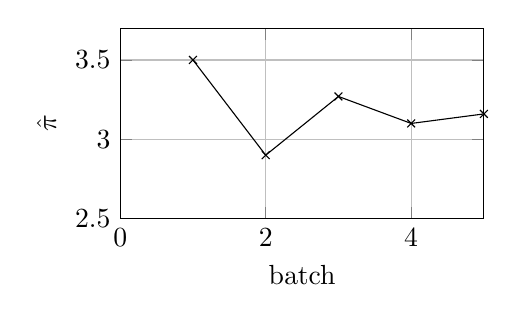
\begin{tikzpicture}
\begin{axis}[width=6.2cm,height=4cm,xmin=0,xmax=5,ymin=2.5,ymax=3.7,grid=major,xlabel={batch},ylabel={$\hat\pi$}]
\addplot[mark=x] coordinates {(1,3.5)(2,2.9)(3,3.27)(4,3.10)(5,3.16)};
\end{axis}
\end{tikzpicture}
\end{center}
\cacographynote{seed recorded?}
Scatter shrinks slowly, roughly $1/\sqrt N$.
\crossout[line]{exact answer} estimate, not proof.
\end{document}
